%------------------------------------------------------------------------------%

\subsubsection{Contexto}

\stopcounter
\begin{frame}{Origem}
  O Freeze-Tag Problem (FTP) surge como um problema de robótica de enxame em 2002~\cite{Arkin02}:
  \bigbreak
  \begin{minipage}{\linewidth}
    \centering
    \multiinclude[format=png, start=0, end=5, graphics={height=5cm}]{FTP/ftp_example/Temp}
  \end{minipage}
\end{frame}
\inccounter

\begin{frame}{Motivação}
  \begin{itemize}[<+->]

    \item Modela problemas de transmissão de dados e design de redes;

    \item Soluções são árvores binárias geradoras de altura mínima;

    \item Ligado às árvores de multicast (estruturas de comunicação da camada de aplicação).

  \end{itemize}
\end{frame}

\begin{frame}{Definição - Instância}
  \begin{itemize}[<+->]

    \item Conjunto de $n$ robôs $R$;

    \item Robô inicial $r_0 \in R$ (\textbf{fonte});

    \item Função de distância $\dist\colon R\times R \to \R^+$.

  \end{itemize}
\end{frame}

\stopcounter
\begin{frame}{Definição - Solução}
  O conjunto de movimentos (\textbf{\emph{schedule}} ou \textbf{árvore de ativação}):

  \pause

  \begin{itemize}[<+->]
    \item Árvore binária $\calt$ enraizada em $r_0$ que visita todos os robôs;

    \item Minimizamos o \textbf{\emph{makespan}}, isto é, o tempo total de ativação.
  \end{itemize}

  \pause
  \bigskip
  \begin{minipage}{\linewidth}
    \centering
    \multiinclude[format=png, start=0, end=5, graphics={height=5cm}]{FTP/solution/Temp}
  \end{minipage}
\end{frame}
\inccounter

%------------------------------------------------------------------------------%

\subsubsection{Resultados Teóricos}

\begin{frame}{Resultado Anterior}
  \begin{thm}[Arkin et al.~\cite{Arkin02}]
    O FTP é fortemente NP-difícil em estrelas com pesos nas arestas.
  \end{thm}
\end{frame}

\begin{frame}{Nossos Resultados}
  \setbeamercolor{block body}{bg=green!35!white}
  \begin{cor}[Pedrosa e Silva~\cite{Pe23}]
    O FTP é NP-difícil em árvores binárias enraizadas, sem pesos nas arestas, com a fonte na raiz e robôs desativados apenas nas folhas.
  \end{cor}

  \pause
  \begin{cor}[Pedrosa e Silva~\cite{Pe23}]
    O FTP é fortemente NP-difícil em árvores ternárias enraizadas, com pesos nas arestas, a fonte na raiz e um robô desativado em cada outro nó.
  \end{cor}
\end{frame}

\begin{frame}{Resultado Anterior}
  \begin{thm}[Arkin et al.~\cite{Arkin02}]
    É NP-difícil aproximar o FTP em grafos com pesos nas arestas dentro de um fator menor que $\nicefrac{5}{3}$, mesmo se o grafo tiver grau máximo $4$ e possuir exatamente um robô em cada nó.
  \end{thm}
\end{frame}

\begin{frame}{Nosso Resultado}
  \setbeamercolor{block body}{bg=green!35!white}
  \begin{thm}
    É NP-difícil aproximar o FTP em grafos sem pesos nas arestas dentro de um fator de até $\nicefrac{3}{2}$, mesmo se o grafo tiver diâmetro $2$ e possuir ao menos um robô em cada nó.
  \end{thm}
\end{frame}

\begin{frame}{Conjectura Inicial}
  \begin{conj}[Arkin et al.~\cite{Arkin06}]
    O FTP é NP-difícil para as distâncias Euclidiana ($L_2$) ou de Manhattan ($L_1$) no plano $\R^2$.
  \end{conj}

  \pause
  Problema 35 do \emph{The Open Problems Project}~\cite{TOPP}.
\end{frame}

\begin{frame}{Resultados Anteriores}
  \begin{thm}[Arkin et al.~\cite{Arkin02}]
    Existe um EPTAS para o FTP com distâncias $L_p$ em qualquer espaço de dimensão fixa $\R^d$, com tempo de execução $O(n \log n) + 2^{O((\overeps)^2\log{\overeps})}$.
  \end{thm}

  \pause
  \begin{thm}[Abel et al.~\cite{Yu17}]
    O FTP é NP-difícil para distância $L_2$ no plano.
  \end{thm}

  \pause
  \begin{thm}[Demaine e Rudoy~\cite{Erik17}]
    O FTP é NP-difícil para distâncias $L_p$, onde $p>1$, em 3D.
  \end{thm}
\end{frame}

\begin{frame}{Nossos Resultados}
  \setbeamercolor{block body}{bg=green!35!white}
  \begin{thm}[Pedrosa e Silva~\cite{Lu23}]
    O FTP é fortemente NP-difícil para distância $L_1$ em 3D.
  \end{thm}

  \pause
  \begin{cor}[Pedrosa e Silva~\cite{Lu23}]
    O FTP é NP-difícil em grades 3D sem pesos nas arestas.
  \end{cor}
\end{frame}

%------------------------------------------------------------------------------%

\subsubsection{Resultados Experimentais}

\begin{frame}{Abordagens Exatas}
  \begin{itemize}[<+->]

    \item Experimentos foram realizados devido à ausência de implementações exatas;

    \item Duas formulações MIP implementadas usando Gurobi;

    \item Uma formulação CP implementada usando o CP-SAT do Google OR-Tools;

    \item Avaliação feita com instâncias usando a distância $L_2$ em $\R^2$.

  \end{itemize}
\end{frame}

\begin{frame}{Tornando um PTAS mais Prático}
  Implementamos o EPTAS de Arkin et al.~\cite{Arkin06}, substituindo a enumeração lenta do algoritmo por nossa formulação CP.

  \bigskip
  \begin{minipage}{\linewidth}
    \centering
    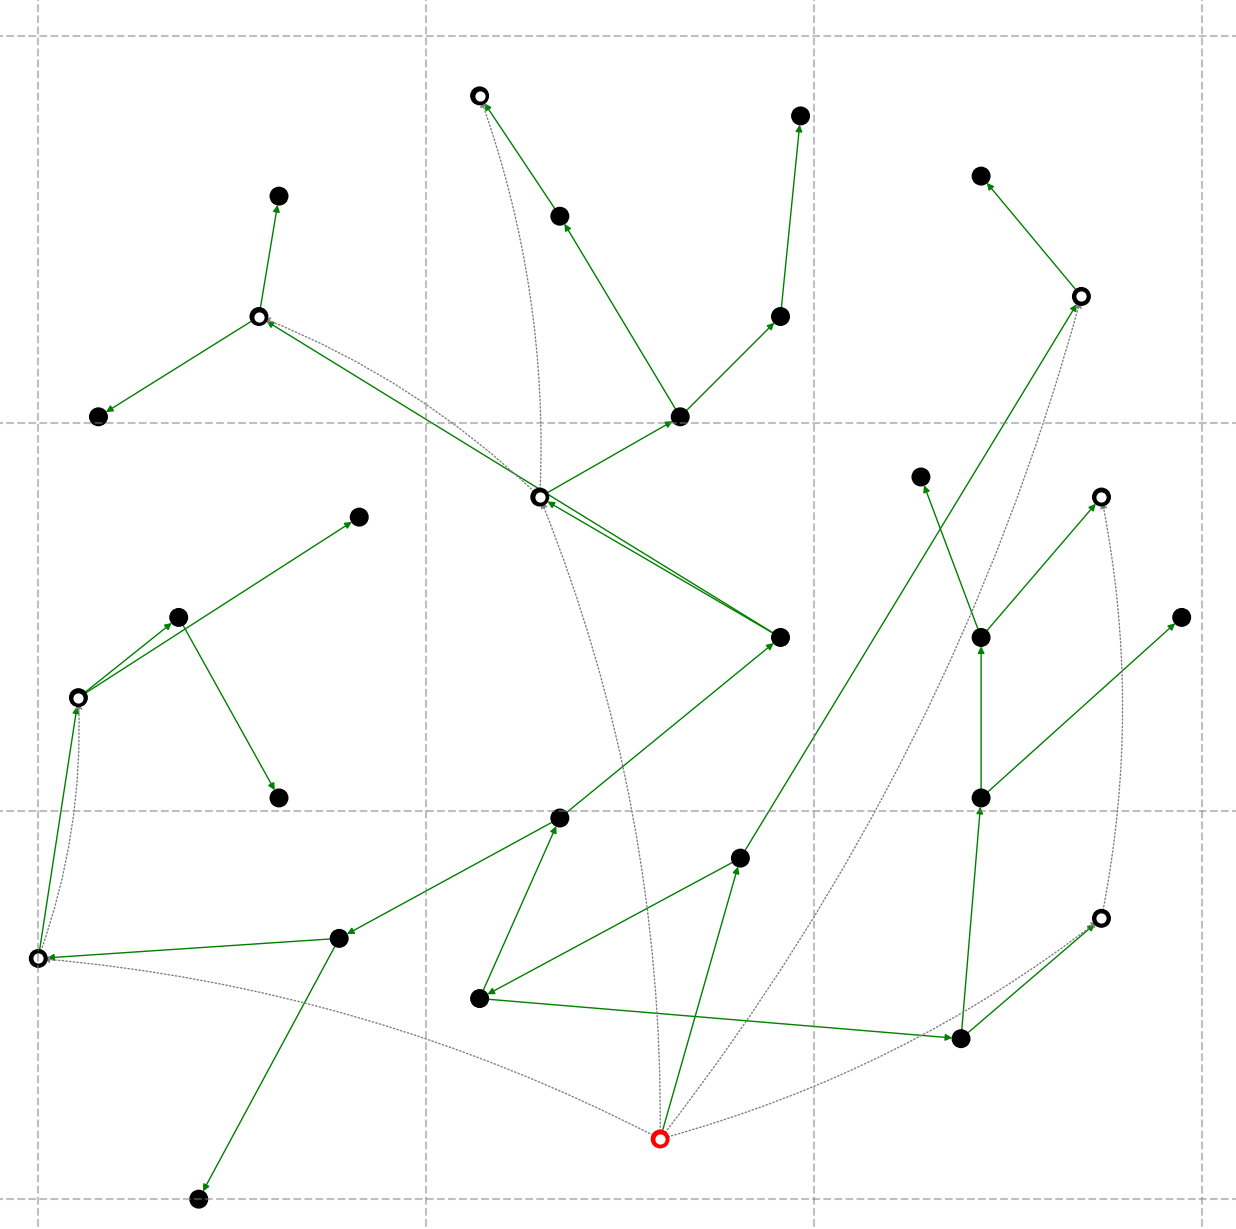
\includegraphics[height=6.7cm]{FTP/ptas_solver.png}
  \end{minipage}
\end{frame}
